\documentclass[journal,12pt,twocolumn]{IEEEtran}

\usepackage{setspace}
\usepackage{gensymb}
\singlespacing
\usepackage[cmex10]{amsmath}
\usepackage{amssymb}
\usepackage{xurl}
\usepackage{tabularx}
\usepackage{amsthm}
\usepackage{comment}
\usepackage{mathrsfs}
\usepackage{txfonts}
\usepackage{stfloats}
\usepackage{bm}
\usepackage{cite}
\usepackage{cases}
\usepackage{subfig}

\usepackage{longtable}
\usepackage{multirow}

\usepackage{enumitem}
\usepackage{mathtools}
\usepackage{steinmetz}
\usepackage{tikz}
\usepackage{circuitikz}
\usepackage{verbatim}
\usepackage{tfrupee}
\usepackage[breaklinks=true]{hyperref}
\usepackage{graphicx}
\usepackage{tkz-euclide}

\usetikzlibrary{calc,math}
\usepackage{listings}
    \usepackage{color}                                            %%
    \usepackage{array}                                            %%
    \usepackage{longtable}                                        %%
    \usepackage{calc}                                             %%
    \usepackage{multirow}                                         %%
    \usepackage{hhline}                                           %%
    \usepackage{ifthen}                                           %%
    \usepackage{lscape}     
\usepackage{multicol}
\usepackage{chngcntr}

\DeclareMathOperator*{\Res}{Res}

\renewcommand\thesection{\arabic{section}}
\renewcommand\thesubsection{\thesection.\arabic{subsection}}
\renewcommand\thesubsubsection{\thesubsection.\arabic{subsubsection}}

\renewcommand\thesectiondis{\arabic{section}}
\renewcommand\thesubsectiondis{\thesectiondis.\arabic{subsection}}
\renewcommand\thesubsubsectiondis{\thesubsectiondis.\arabic{subsubsection}}


\hyphenation{op-tical net-works semi-conduc-tor}
\def\inputGnumericTable{}                                 %%

\lstset{
%language=C,
frame=single, 
breaklines=true,
columns=fullflexible
}
\begin{document}


\newtheorem{theorem}{Theorem}[section]
\newtheorem{problem}{Problem}
\newtheorem{proposition}{Proposition}[section]
\newtheorem{lemma}{Lemma}[section]
\newtheorem{corollary}[theorem]{Corollary}
\newtheorem{example}{Example}[section]
\newtheorem{definition}[problem]{Definition}

\newcommand{\BEQA}{\begin{eqnarray}}
\newcommand{\EEQA}{\end{eqnarray}}
\newcommand{\define}{\stackrel{\triangle}{=}}
\bibliographystyle{IEEEtran}
\raggedbottom
\setlength{\parindent}{0pt}
\providecommand{\mbf}{\mathbf}
\providecommand{\pr}[1]{\ensuremath{\Pr\left(#1\right)}}
\providecommand{\qfunc}[1]{\ensuremath{Q\left(#1\right)}}
\providecommand{\sbrak}[1]{\ensuremath{{}\left[#1\right]}}
\providecommand{\lsbrak}[1]{\ensuremath{{}\left[#1\right.}}
\providecommand{\rsbrak}[1]{\ensuremath{{}\left.#1\right]}}
\providecommand{\brak}[1]{\ensuremath{\left(#1\right)}}
\providecommand{\lbrak}[1]{\ensuremath{\left(#1\right.}}
\providecommand{\rbrak}[1]{\ensuremath{\left.#1\right)}}
\providecommand{\cbrak}[1]{\ensuremath{\left\{#1\right\}}}
\providecommand{\lcbrak}[1]{\ensuremath{\left\{#1\right.}}
\providecommand{\rcbrak}[1]{\ensuremath{\left.#1\right\}}}
\theoremstyle{remark}
\newtheorem{rem}{Remark}
\newcommand{\sgn}{\mathop{\mathrm{sgn}}}
\providecommand{\abs}[1]{\vert#1\vert}
\providecommand{\res}[1]{\Res\displaylimits_{#1}} 
\providecommand{\norm}[1]{\lVert#1\rVert}
%\providecommand{\norm}[1]{\lVert#1\rVert}
\providecommand{\mtx}[1]{\mathbf{#1}}
\providecommand{\mean}[1]{E[ #1 ]}
\providecommand{\fourier}{\overset{\mathcal{F}}{ \rightleftharpoons}}
%\providecommand{\hilbert}{\overset{\mathcal{H}}{ \rightleftharpoons}}
\providecommand{\system}{\overset{\mathcal{H}}{ \longleftrightarrow}}
	%\newcommand{\solution}[2]{\textbf{Solution:}{#1}}
\newcommand{\solution}{\noindent \textbf{Solution: }}
\newcommand{\cosec}{\,\text{cosec}\,}
\providecommand{\dec}[2]{\ensuremath{\overset{#1}{\underset{#2}{\gtrless}}}}
\newcommand{\myvec}[1]{\ensuremath{\begin{pmatrix}#1\end{pmatrix}}}
\newcommand{\mydet}[1]{\ensuremath{\begin{vmatrix}#1\end{vmatrix}}}
\newcommand*{\permcomb}[4][0mu]{{{}^{#3}\mkern#1#2_{#4}}}
\newcommand*{\perm}[1][-3mu]{\permcomb[#1]{P}}
\newcommand*{\comb}[1][-1mu]{\permcomb[#1]{C}}
\numberwithin{equation}{subsection}
\makeatletter
\@addtoreset{figure}{problem}
\makeatother
\let\StandardTheFigure\thefigure
\let\vec\mathbf
\renewcommand{\thefigure}{\theproblem}
\def\putbox#1#2#3{\makebox[0in][l]{\makebox[#1][l]{}\raisebox{\baselineskip}[0in][0in]{\raisebox{#2}[0in][0in]{#3}}}}
     \def\rightbox#1{\makebox[0in][r]{#1}}
     \def\centbox#1{\makebox[0in]{#1}}
     \def\topbox#1{\raisebox{-\baselineskip}[0in][0in]{#1}}
     \def\midbox#1{\raisebox{-0.5\baselineskip}[0in][0in]{#1}}
\vspace{3cm}
\title{AI1103 : Assignment 2}
\author{Raja Ravi Kiran Reddy- CS20BTECH11009}
\maketitle
\newpage
\bigskip
\renewcommand{\thefigure}{\arabic{figure}}
\renewcommand{\thetable}{\arabic{table}}
Download all python codes from 
\begin{lstlisting}
https://github.com/BokkaRajaRaviKiranReddy/AI1103/tree/main/Assignment2/codes
\end{lstlisting}
%
and latex codes from 
%
\begin{lstlisting}
https://github.com/BokkaRajaRaviKiranReddy/AI1103/blob/main/Assignment2/Assignment2.tex
\end{lstlisting}
\section*{GATE 2020 EC-Q54}
X is a random variable with uniform probability density function in the interval
 [−2,10] .For Y=2X-6,The conditional probability P$(Y\leq7|X\geq5)$
(rounded off to three decimal places) is 
\section*{Solution}
\begin{align*}
\tag{54.1}
  &\Pr(Y\leq7|X\geq5)=\frac{\Pr(Y\leq7,X\geq5)}{\Pr(X\geq5)}\\
  &X=\frac{Y+6}{2}\geq5\\
  &\implies Y+6\geq10\\
  &\implies Y\geq4
\end{align*}
So,  From Equation 54.1
\begin{align}
   \tag{54.2}
   \Pr(Y\leq7|X\geq5)=\frac{\Pr(Y\leq7,Y\geq4)}{\Pr(X\geq5)}
\end{align}
As $X\in [-2,10]$ with uniform probability density function,\\
PDF oF X is

\begin{align}
\tag{54.3}
 &f_X(x)=\begin{cases}
  \dfrac{1}{12}  \text{  if} -2\leq x \leq10\\
    0 \text{  otherwise}
  \end{cases}
\end{align}
\begin{figure}[h]
    \centering
    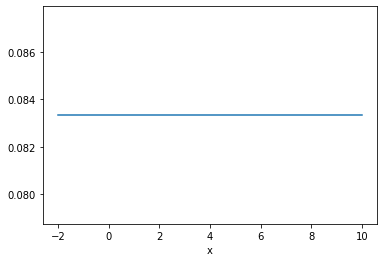
\includegraphics[width=\columnwidth]{PDFofX.png}
    \caption{PDF of X}
    \label{fig:my_label}
\end{figure}

Given Y=2X-6
$\implies Y \in [-10,14] $\\
So, PDF of Y is 
\begin{align}
 \tag{54.4}
  f_Y(y)=\begin{cases}
  \dfrac{1}{24} \text{ if} -10\leq y \leq 14\\
  0  \text{   otherwise}
  \end{cases}
\end{align}\\
\begin{figure}[h]
    \centering
    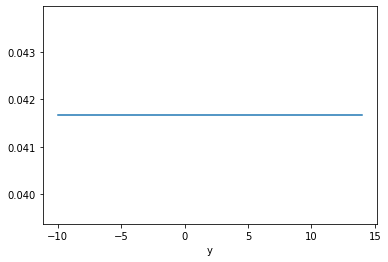
\includegraphics[width=\columnwidth]{PDFofY.png}
    \caption{PDF of Y}
    \label{fig:my_label}
\end{figure}

CDF of X,
\begin{align*}
    &F_X(x)=\int_{-\infty}^{x}f_X(x)\,dx
\end{align*}
\begin{align*}
  F_X(x)=\begin{cases}
  0  \text{ if } x\leq-2\\
  \dfrac{1}{12}(x+2) \text{ if} -2\leq x \leq 10\\
  1 \text{  if }  x \geq 10
  \end{cases}
\end{align*}
CDF of Y,
\begin{align*}
    &F_Y(y)=\int_{-\infty}^{y}f_Y(y)\,dx
\end{align*}
\begin{align*}
  F_y(y)=\begin{cases}
  0  \text{ if } y\leq-10\\
  \dfrac{1}{24}(y+10) \text{ if} -10\leq y \leq 14\\
  1 \text{  if }  y \geq 14
  \end{cases}
\end{align*}

So,  From Equation 54.2
\begin{align*}
&\Pr(Y\leq7|X\geq5)=\frac{\Pr(Y\leq7,Y\geq4)}{\Pr(X\geq5,X\leq10)}\\
&=\frac{F_Y(7)-F_Y(4)}{F_X(10)-F_X(5)}\\
&=\frac{\dfrac{17}{24}-\dfrac{14}{24}}{\dfrac{12}{12}-\dfrac{7}{12}}\\
&=0.300
\end{align*}
\begin{figure}[h]
    \centering
    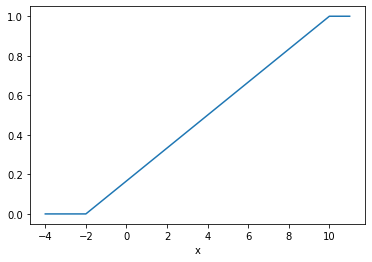
\includegraphics[width=\columnwidth]{CDFofX.png}
    \caption{CDF of X}
    \label{fig:my_label}
\end{figure}

\begin{figure}[h]
    \centering
    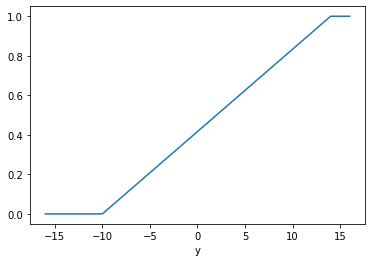
\includegraphics[width=\columnwidth]{CDFofY.png}
    \caption{CDF of Y}
    \label{fig:my_label}
\end{figure}



\end{document}
